%!TEX root = ../../thesis.tex

\Section~\ref{sec:signature} outlined the basic experimental signature of the search as 
two oppositely charged leptons and significant \met. Thus, the initial stages of the 
event selection are tasked with finding this signature. Subsequent criteria, or 
\textit{cuts}, target specific backgrounds. Their aim is improve the analysis sensitivity 
by suppressing backgrounds whilst retaining a sufficient number of signal events.



\subsection{Data quality}
\label{sec:selection:quality}

The \pp dataset (see \Section~\ref{sec:dataset:dataset}) is hierarchically split into 
\textit{periods} of broadly consistent beam conditions, \textit{runs} typically 
corresponding to LHC fills, and \textit{luminosity blocks} of \about 2~minutes where the 
instantaneous luminosity is approximately constant. Luminosity blocks are included in the 
analysis if the detector was operating sufficiently for the recorded data to be 
considered `good for physics' (see \Figure~\ref{fig:dataset:lumi}).\footnote{
	ATLAS good runs list: \texttt{data12\symbol{95}8TeV.periodAllYear\symbol{95}DetStatus-v61-pro14-02\symbol{95}DQDefects-00-01
	-00\symbol{95}PHYS\symbol{95}StandardGRL\symbol{95}All\symbol{95}Good.xml}
} 
For the 2012 dataset, this corresponds to a total integrated luminosity of 
\unit{20.3}{\invfb}.

Individual events are also vetoed if certain data quality criteria are failed by:
\begin{itemize}[noitemsep,nolistsep]
	\item a noise burst in the LAr calorimeter,
	\item data corruption caused by a restart of the synchronisation system,
	\item a \textit{looser} jet is reconstructed with \pt $>$ \unit{20}{\GeV} (indicative of an HCal spike),
	\item a jet is reconstructed near a `hot' HCal tile (1st -- 8th May 2012 only).
\end{itemize}
A further quality criterion requires that the primary vertex considered as the hard 
scatter (that with the highest $\sum p_{\text{T}}^2$) must be associated with at least 
three tracks. This reduces the cosmic ray background to negligible levels.



\subsection{Trigger}
\label{sec:selection:trigger}

It is infeasible to record all events in the \unit{20.3}{\invfb} dataset; ATLAS instead 
employs a trigger system to identify and record interesting events (see 
\Section~\ref{sec:atlas:trig}). In the \HWWlvlv search it is natural to trigger on 
high-\pt leptons, using algorithms similar to, though less sophisticated than, those in 
\Section~\ref{sec:objects:electrons} and \Section~\ref{sec:objects:muons}.

A trigger is characterised by its efficiency versus \pt curve (though it also depends on 
$\eta$), which has a turn-on followed by a plateau, as shown in 
\Figure~\ref{fig:sel:trig_eff}. It is preferable to operate on the plateau, where the 
efficiency is more stable. To maximise the signal yield, it is desirable to use a trigger 
with a lower turn-on \pt. However, increased backgrounds and limitations to trigger 
latency and bandwidth require a compromise to be found. The lowest unprescaled\footnote{
	A \textit{prescaled} trigger reduces the turn-on \pt by recording only 1 in $N$ 
	events passing the trigger, and weighting such events by a factor $N$. In doing so, 
	some statistical power is lost.
}
single lepton triggers available in 2012 had nominal \pt thresholds of \unit{24}{\GeV}. 
Fortunately, it is possible to recover trigger efficiency at low-\pt by using dilepton 
triggers, because the backgrounds are much smaller.

\begin{figure}
	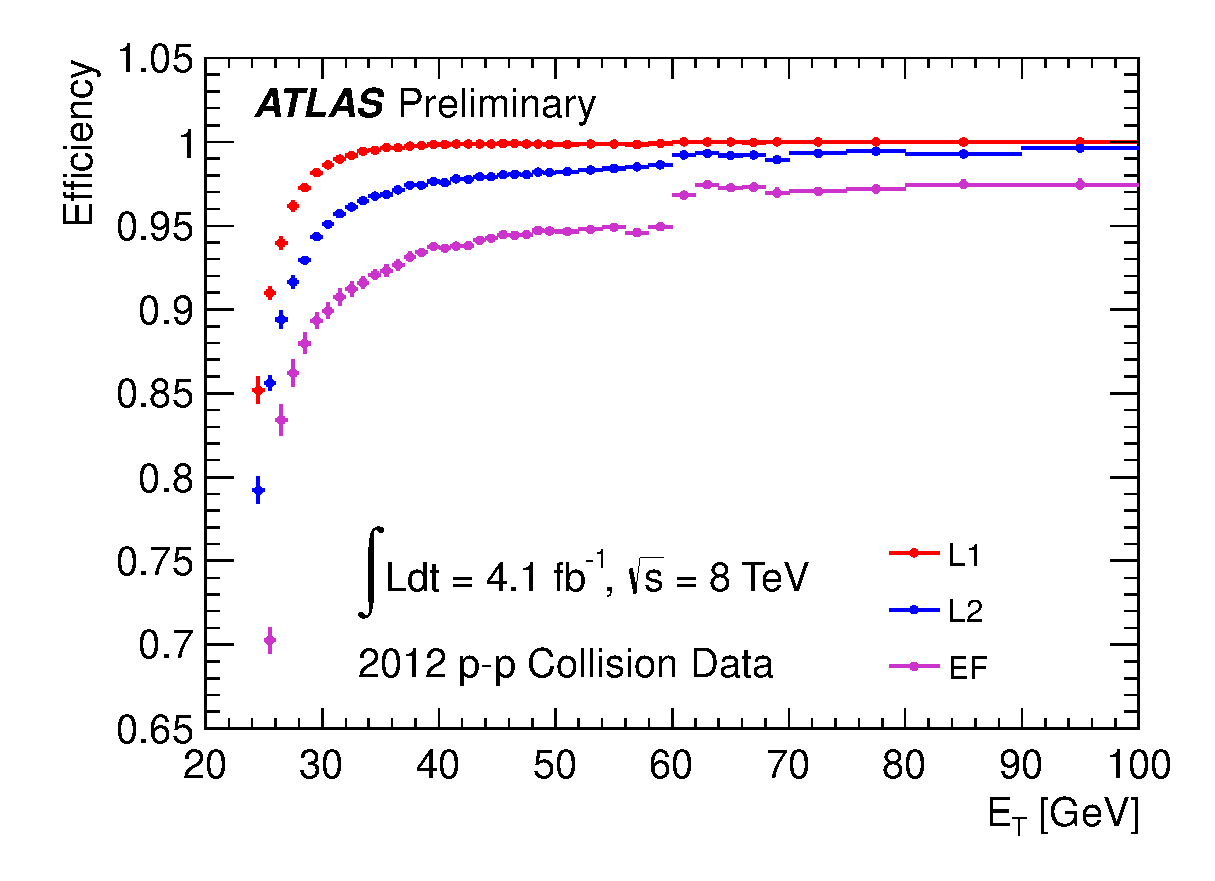
\includegraphics[width=0.495\textwidth]{tex/selection/trigger_eff_el}
	\hfill
	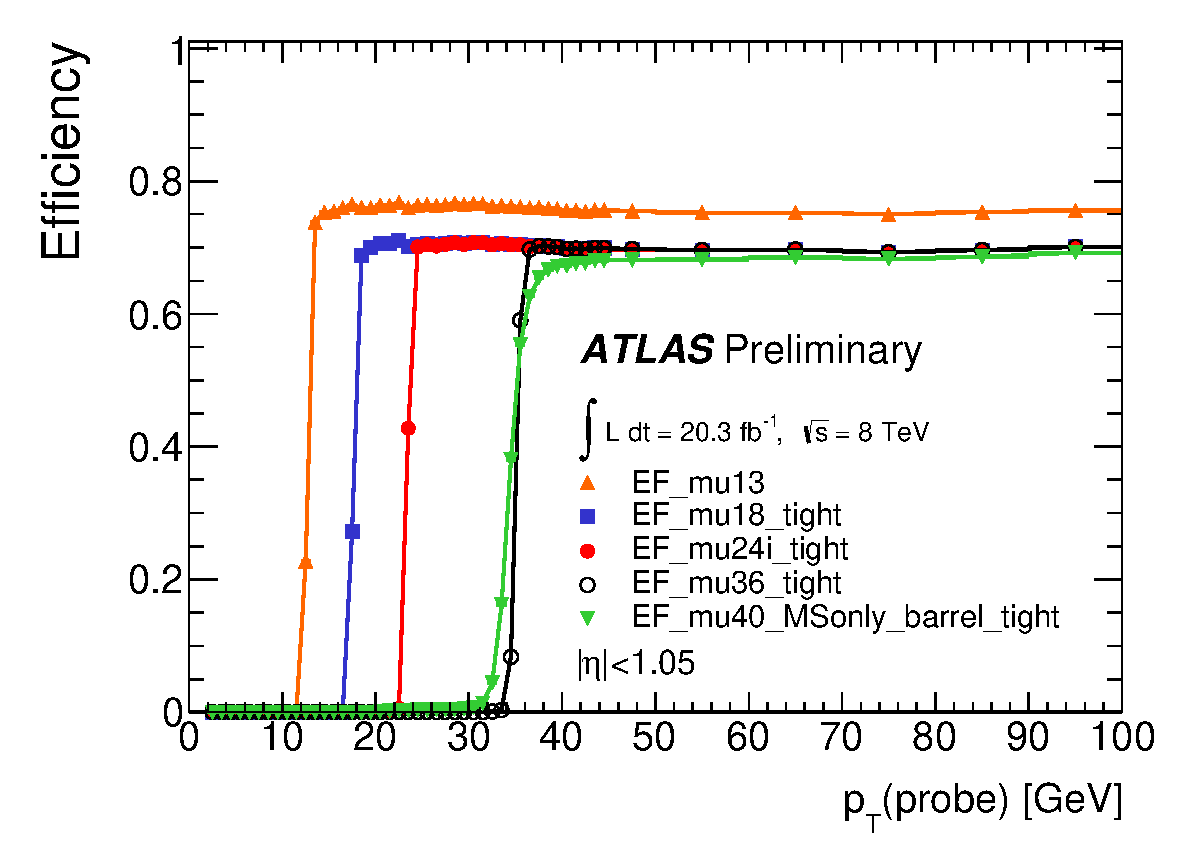
\includegraphics[width=0.495\textwidth]{tex/selection/trigger_eff_mu}
	\caption{Efficiencies of the single lepton triggers for electrons with respect to 
	offline \textit{medium} identification (left) and muons with respect to offline 
	reconstruction (right).}
	\label{fig:sel:trig_eff}
\end{figure}

Events are required to pass at least one trigger listed in \Table~\ref{tab:sel:triggers}. 
The single lepton triggers include a tighter low-\pt trigger and a looser high-\pt 
trigger in order to maximise the efficiency. Dilepton triggers are then used to increase 
the efficiency during the turn-on of the single lepton triggers. Together, these triggers 
support a \pt threshold of \unit{22}{\GeV} on the leading lepton (in the 
offline analysis), whilst operating on the plateau.

\begin{table}
	\begin{tabular}{lllcl}
		\multirow{2}{2.5cm}{Single lepton triggers} & \Pe  & \verb|EF_e24vhi_medium1| & or & \verb|EF_e60_medium1| \\
		& \Pmu & \verb|EF_mu24i_tight| & or & \verb|EF_mu36_tight|  \\
		\hline
		\multirow{3}{2.5cm}{Dilepton triggers} & \HepProcess{\Pe\Pe} & \verb|EF_2e12Tvh_loose1| & or & \verb|EF_2e12Tvh_loose1_L2StarB| \\
		& \HepProcess{\Pmu\Pmu} & \multicolumn{3}{l}{\texttt{EF\symbol{95}mu18\symbol{95}tight\symbol{95}mu8\symbol{95}EFFS}} \\
		& \HepProcess{\Pe\Pmu}  & \multicolumn{3}{l}{\texttt{EF\symbol{95}e12Tvh\symbol{95}medium1\symbol{95}mu8}} \\
	\end{tabular}
	\caption{Employed trigger names. \texttt{EF} refers to event filter, \texttt{e} is an 
	electron, \texttt{mu} is a muon, the following number is the \pt threshold, 
	\texttt{vh} indicates calorimeter isolation, \texttt{i} indicates track isolation, 
	and \texttt{tight}, \texttt{medium} or \texttt{loose} is the identification. Other 
	parts relate to the trigger chain. Criteria are looser than those applied 
	offline.}
	\label{tab:sel:triggers}
\end{table}

Trigger efficiencies are measured via tag-and-probe of 
\HepProcess{\PZ \HepTo \Plepton\Plepton} events, where the tag and probe have both 
passed the offline lepton selection and the tag has successfully matched to a triggered 
lepton object. For example, single lepton trigger efficiencies are displayed in 
\Figure~\ref{fig:sel:trig_eff}. Comparison with MC yields efficiency scale factors.

Additionally, events are required to have at least one lepton passing the offline 
reconstruction that is matched within $\Delta R < 0.15$ of a triggered lepton object.
Single lepton triggers are matched to offline leptons with $\pt > \unit{25}{\GeV}$. On 
the other hand, dilepton triggers comprise two triggered objects: \texttt{mu8} is matched 
to offline muons with $\pt > \unit{10}{\GeV}$, \texttt{mu18} is matched to offline muons 
with $\pt > \unit{20}{\GeV}$, and \texttt{e12} is matched to offline electrons with 
$\pt > \unit{15}{\GeV}$.



\subsection{Preselection of dilepton + \met signature}
\label{sec:selection:presel}

Following the trigger selection, events are required to have two oppositely charged 
leptons passing the offline selection (see \Section~\ref{sec:objects}). The lepton with 
the highest \pt, called the \textit{leading lepton}, must have 
\unit{$\ptleadlep > 22$}{\GeV} in order to operate on the trigger plateau. The 
\textit{subleading lepton} must have \unit{$\ptsubleadlep > 10$}{\GeV}, as specified in 
\Section~\ref{sec:objects}. Events containing a third lepton are vetoed in order to 
reject backgrounds with three or more leptons in the final state, such as \WZ production.

At this point, it is possible to split the dilepton final state into four channels 
according to the flavours of the two leptons: \ee, \mm, \em, \me (where the first flavour 
is that of the leading lepton). This is very useful because the background compositions 
of the channels are dramatically different. For example, the \DY background is much 
larger in the same flavour channels (\ee/\mm) than the different flavour channels 
(\em/\me).

Low mass hadronic resonances with dileptonic decays (\eg \PJpsi) are removed from the 
\ee/\mm channels by requiring the mass of the dilepton system \unit{$\mll > 12$}{\GeV}. 
This also greatly suppresses the low mass \DY background. For the \em/\me channels, 
a cut of \unit{$\mll > 10$}{\GeV} suppresses leptons from heavy flavour decays. The 
\ee/\mm channels are hugely dominated by the \DY background (see 
\Figure~\ref{fig:sel:mll}), but a large fraction of these events can be rejected by 
vetoing a window around the \PZ mass, \unit{$\mods{\mll - \mZ} > 15$}{\GeV}.

\begin{figure}
	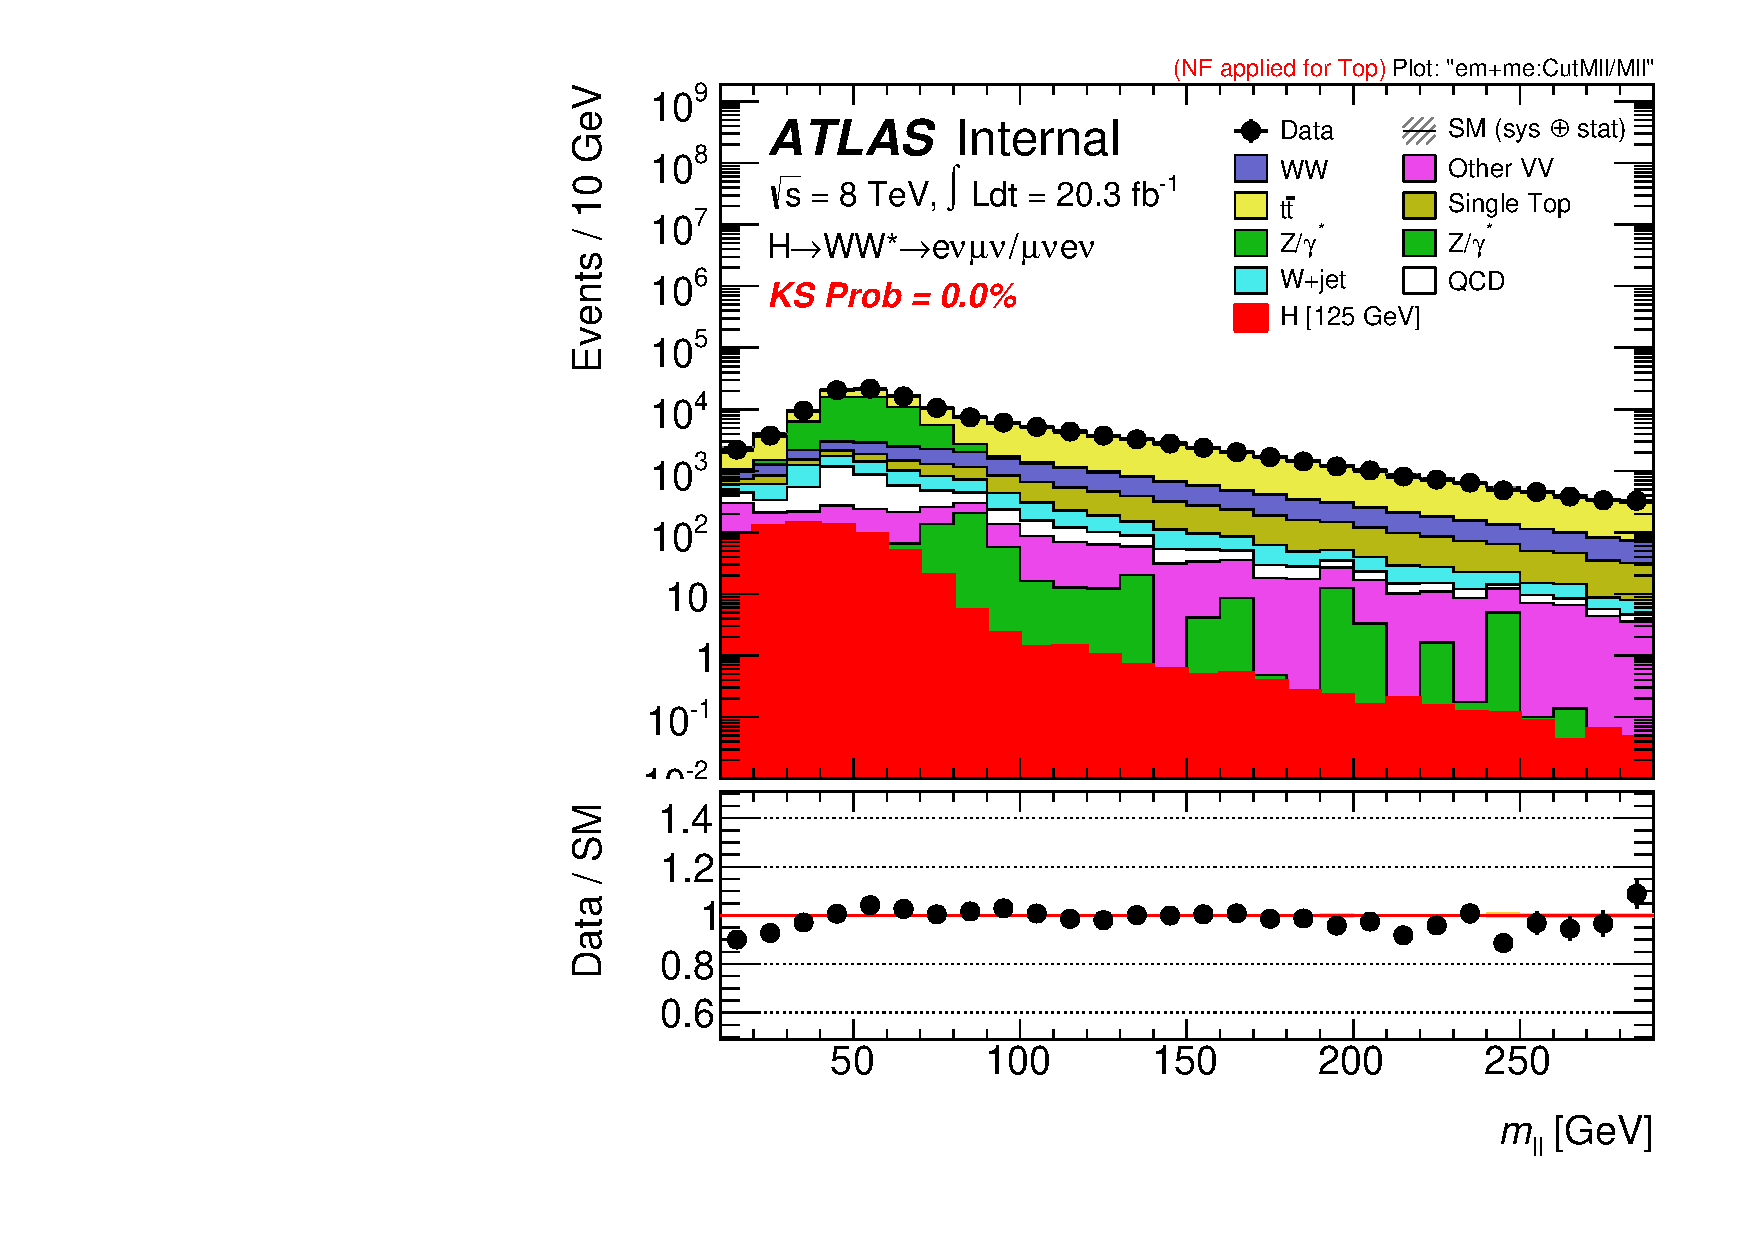
\includegraphics[width=0.495\textwidth]{tex/selection/emme_CutMll_Mll_mh125_log}
	\hfill
	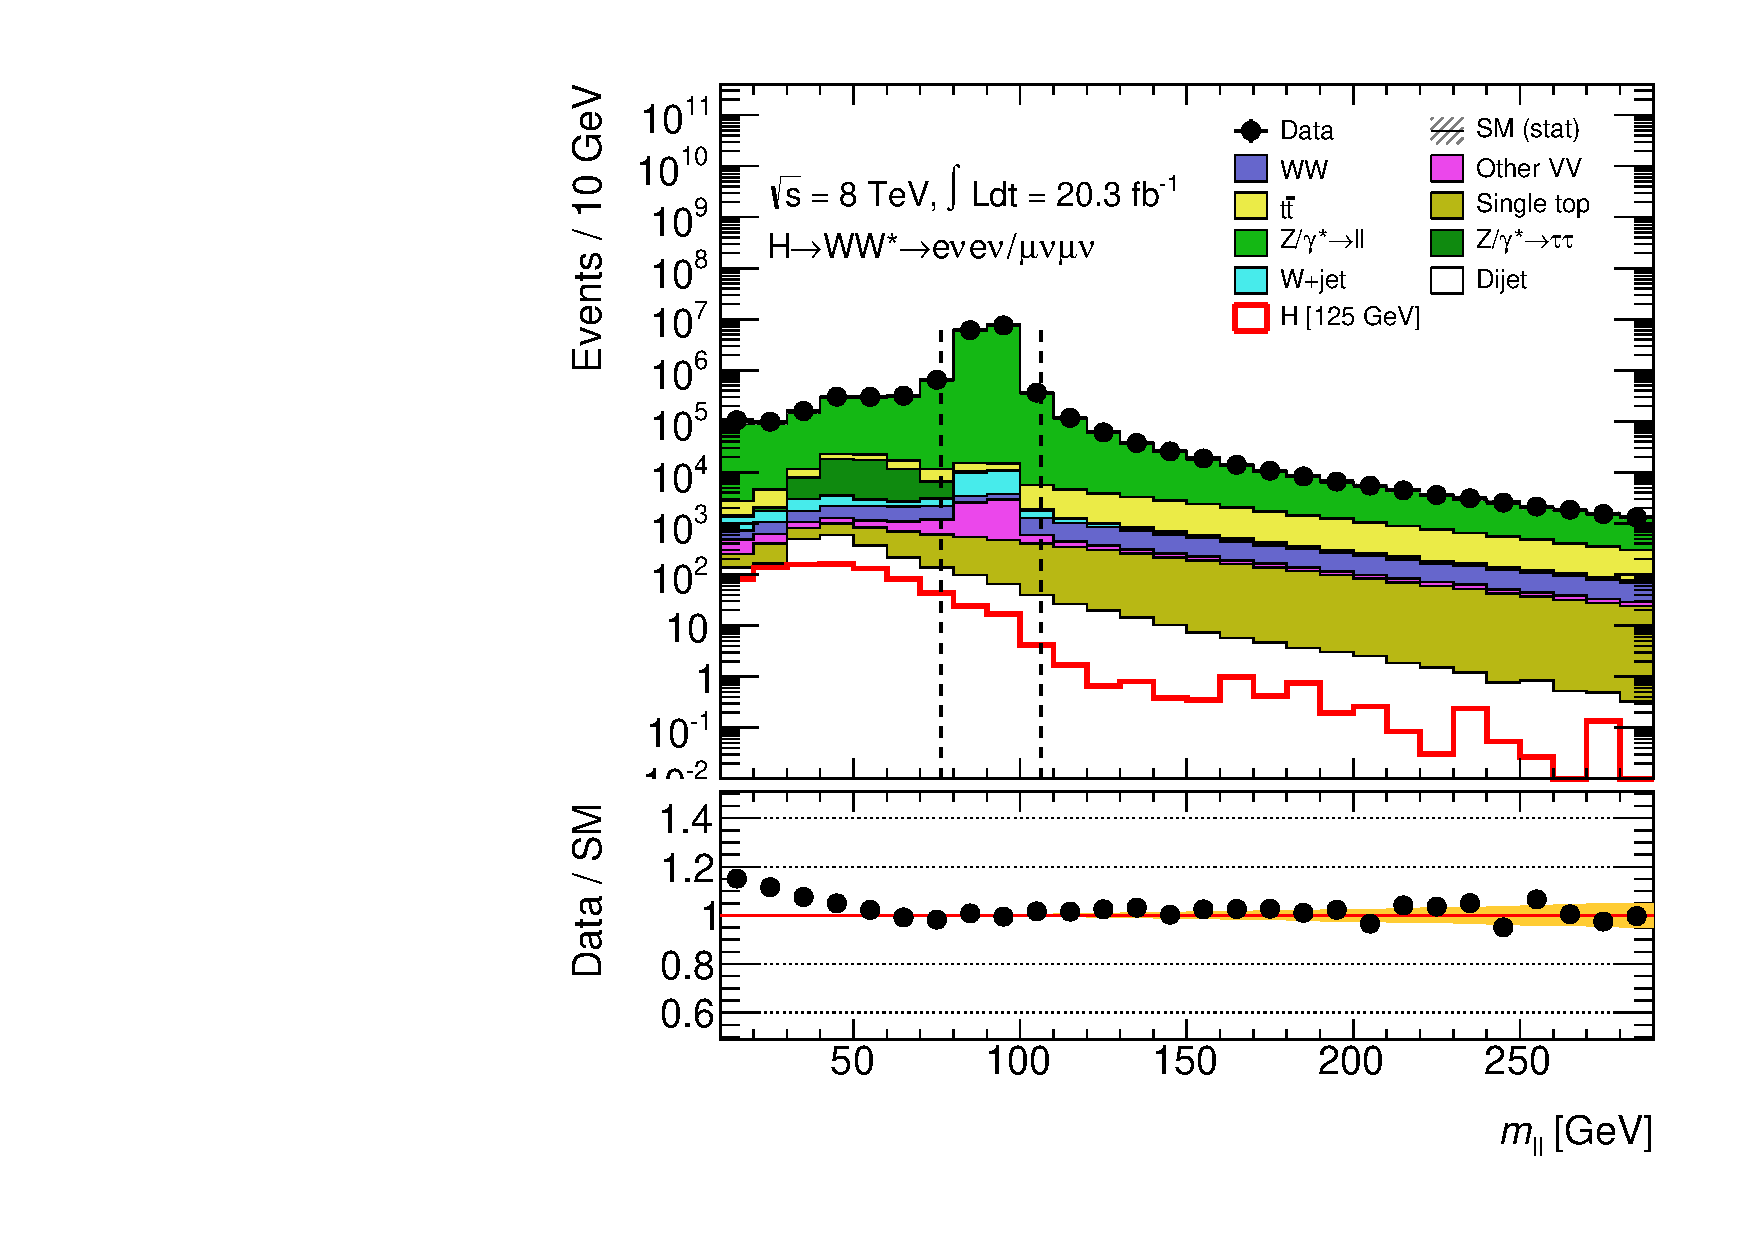
\includegraphics[width=0.495\textwidth]{tex/selection/eemm_CutMll_Mll_mh125_log}
	\caption{Dilepton mass distribution directly preceding the \PZ mass veto, in the 
	\em/\me (left) and \ee/\mm (right) channels. \todo[inline]{update and add cut lines}}
	\label{fig:sel:mll}
\end{figure}



\begin{figure}
	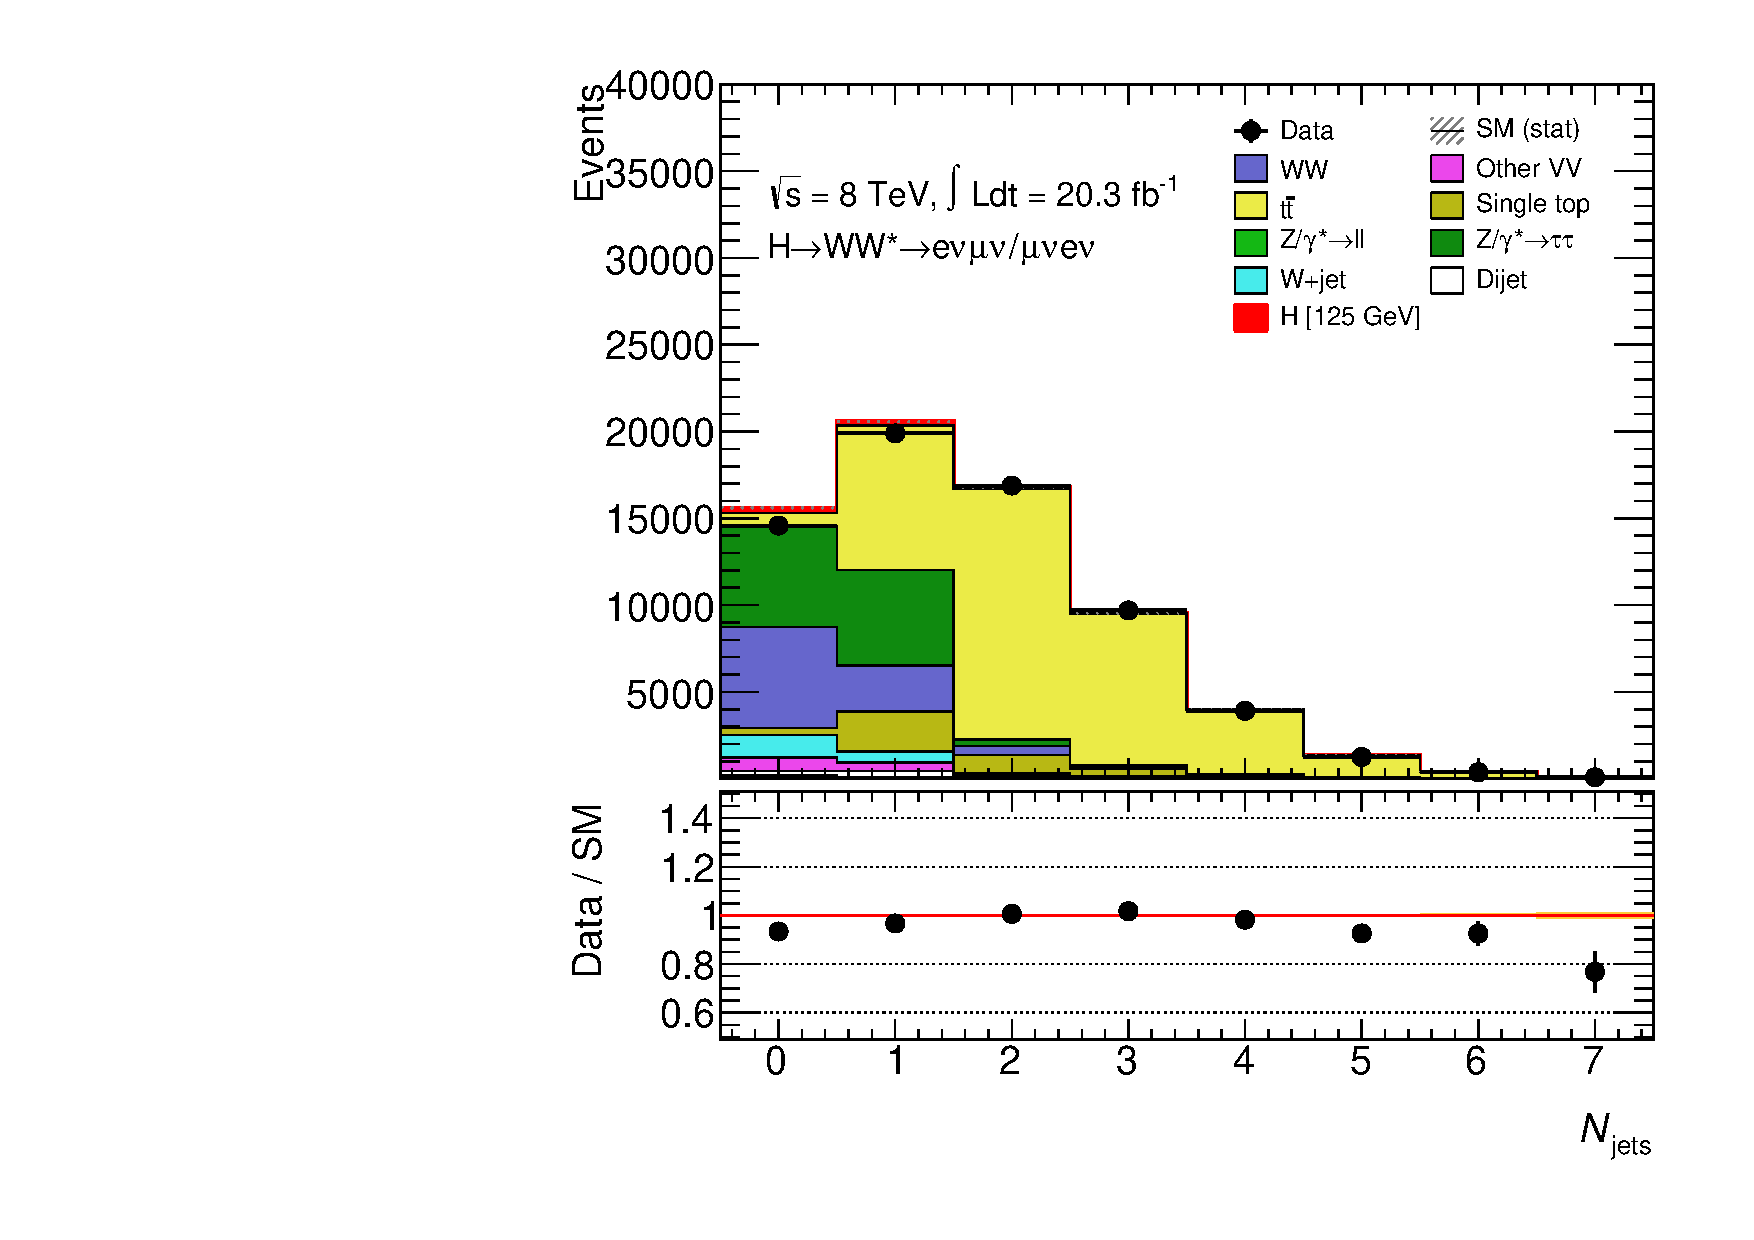
\includegraphics[width=0.495\textwidth]{tex/selection/emme_CutMETRel_m_jet_n_upTo7_mh125_lin}
	\hfill
	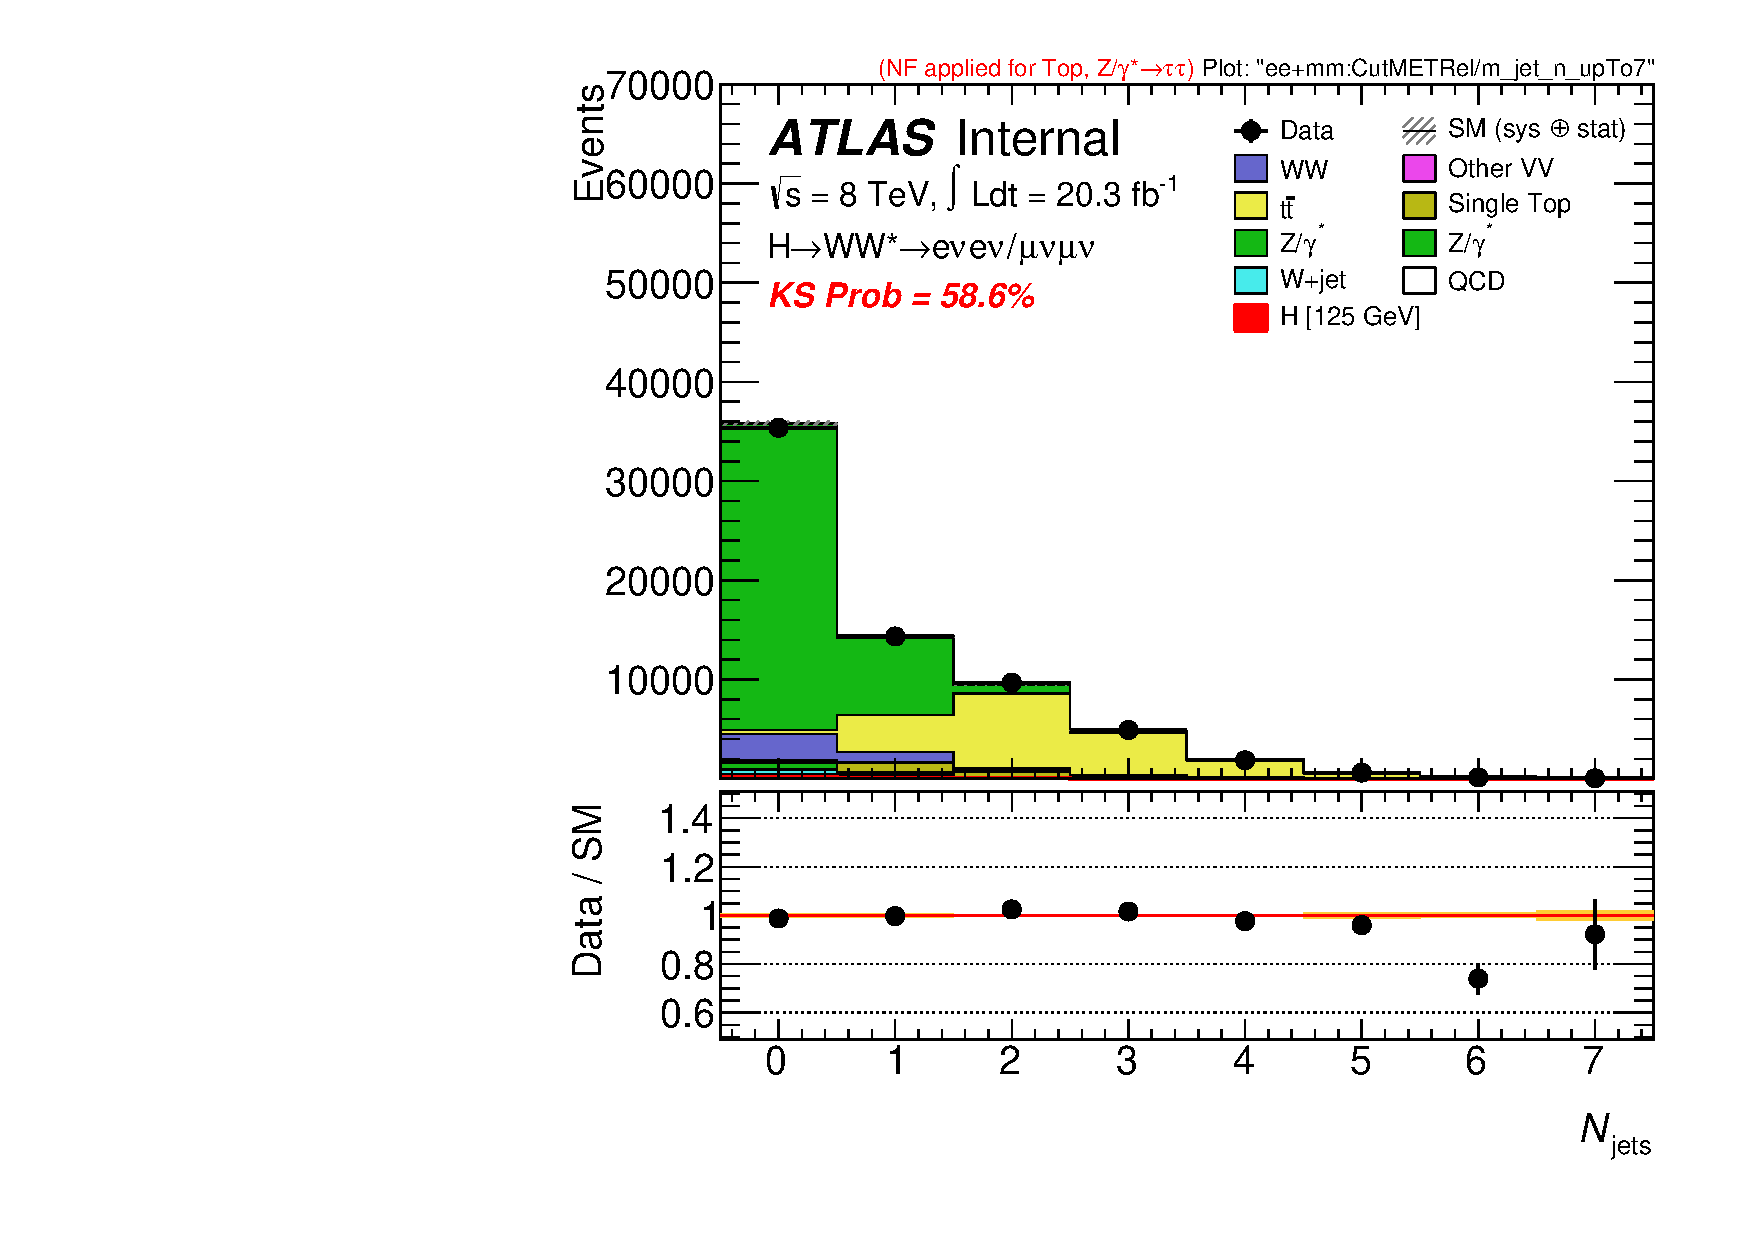
\includegraphics[width=0.495\textwidth]{tex/selection/eemm_CutMETRel_m_jet_n_upTo7_mh125_lin}
	\caption{Jet multiplicity distribution directly preceding jet binning, in the 
	\em/\me (left) and \ee/\mm (right) channels.}
	\label{fig:sel:njets}
\end{figure}


\subsection{0-jet selection}
\label{sec:selection:0j}

\subsection{1-jet selection}
\label{sec:selection:1j}

\subsection{\twojet selection}
\label{sec:selection:2j}

\subsection{Summary}
\label{sec:selection:summary}

\begin{table}
	\begin{tabular}{cc}
		\em/\me & \ee/\mm \\
		\hline
		\multicolumn{2}{c}{\ptleadlep $>$ \unit{22}{\GeV}} \\
		\mll $>$ \unit{10}{\GeV} & \mll $>$ \unit{12}{\GeV} \\
		-- & $\mods{\mll - \mZ} > $ \unit{15}{\GeV} \\
		\hline
		% 0 JET
		\multicolumn{2}{c}{0-jet selection} \\
		\hline
		\corrtrackmet $>$ \unit{20}{\GeV} & \metrel $>$ \unit{40}{\GeV} \\
		\multicolumn{2}{c}{\njets $=$ 0} \\
		\multicolumn{2}{c}{\dphillmet $> \pi/2$} \\
		\multicolumn{2}{c}{\ptll $>$ \unit{30}{\GeV}} \\
		\multicolumn{2}{c}{\mll $<$ \unit{55}{\GeV}} \\
		-- & \trackmet $>$ \unit{40}{\GeV} \\
		\multicolumn{2}{c}{\dphill $<$ 1.8} \\
		-- & \frecoil $<$ 0.1 \\
		\hline
		% 1 JET
		\multicolumn{2}{c}{1-jet selection} \\
		\hline
		\corrtrackmet $>$ \unit{10}{\GeV} & \metrel $>$ \unit{40}{\GeV} \\
		\multicolumn{2}{c}{\njets $=$ 1} \\
		\multicolumn{2}{c}{\nbjets $=$ 0} \\
		$\max\parenths{\mt{\Plepton_1}, \mt{\Plepton_2}} >$ \unit{50}{\GeV} & -- \\
		$m_{\Ptau\Ptau} < \mZ - \unit{25}{\GeV}$ & -- \\
		\multicolumn{2}{c}{\mll $<$ \unit{55}{\GeV}} \\
		-- & \trackmet $>$ \unit{35}{\GeV} \\
		\multicolumn{2}{c}{\dphill $<$ 1.8} \\
		-- & \frecoil $<$ 0.1 \\
	\end{tabular}
	\caption{Summary}
	\label{tab:selection}
\end{table}